\chapter{Introduction}

The interest of natural scientists in social phenomena has been present for a long time. In the late twentieth century it became clear that some social and economic systems can be studied effectively using tools from theoretical physics, especially statistical physics. This observation helped give rise to the field known as \emph{econophysics}. The term was introduced by H. Eugene Stanley at a conference in Kolkata in 1995.

By the end of the 1990s many physicists and mathematicians were working on economic and financial problems. For example, a Nature report noted that a large fraction of doctoral graduates in physics and mathematics (48 \%) took jobs in finance.\cite{gershon1998bank}

Econophysics applies methods from theoretical physics, especially statistical physics, to the study of financial markets and related economic phenomena, which are treated as complex systems. The aim is to build simple, testable models that capture collective effects emerging from the interactions of many agents, following a \textit{data-driven} approach.

A simple illustration of the analogy between a physical and a financial process is the resemblance between Brownian motion and the time series of asset prices. Compare (a) a one-dimensional projection of a Brownian particle's trajectory with (b) an example spot-price time series.

\begin{figure}[htbp]
\centering
% Cambia [b] in [t] per allineare i grafici in alto
\begin{subfigure}[t]{0.48\textwidth}
    \centering
    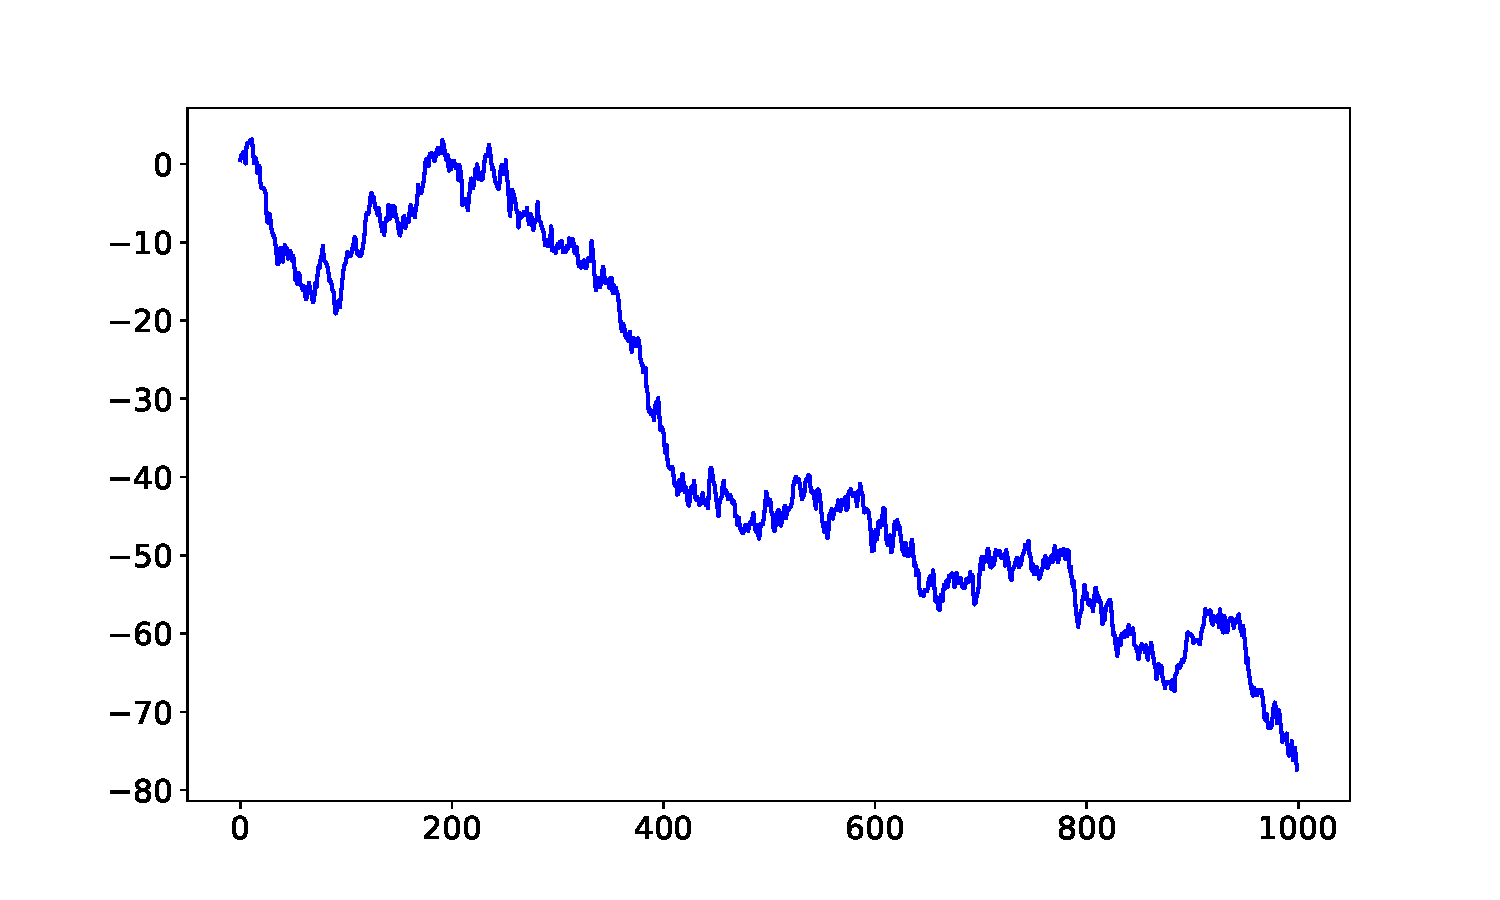
\includegraphics[width=\linewidth]{images/brownian_motion_1d.pdf}
    \caption{One-dimensional Brownian motion (sample path)}
    \label{fig:brownian}
\end{subfigure}\hfill
% Cambia [b] in [t] anche qui
\begin{subfigure}[t]{0.48\textwidth}
    \centering
    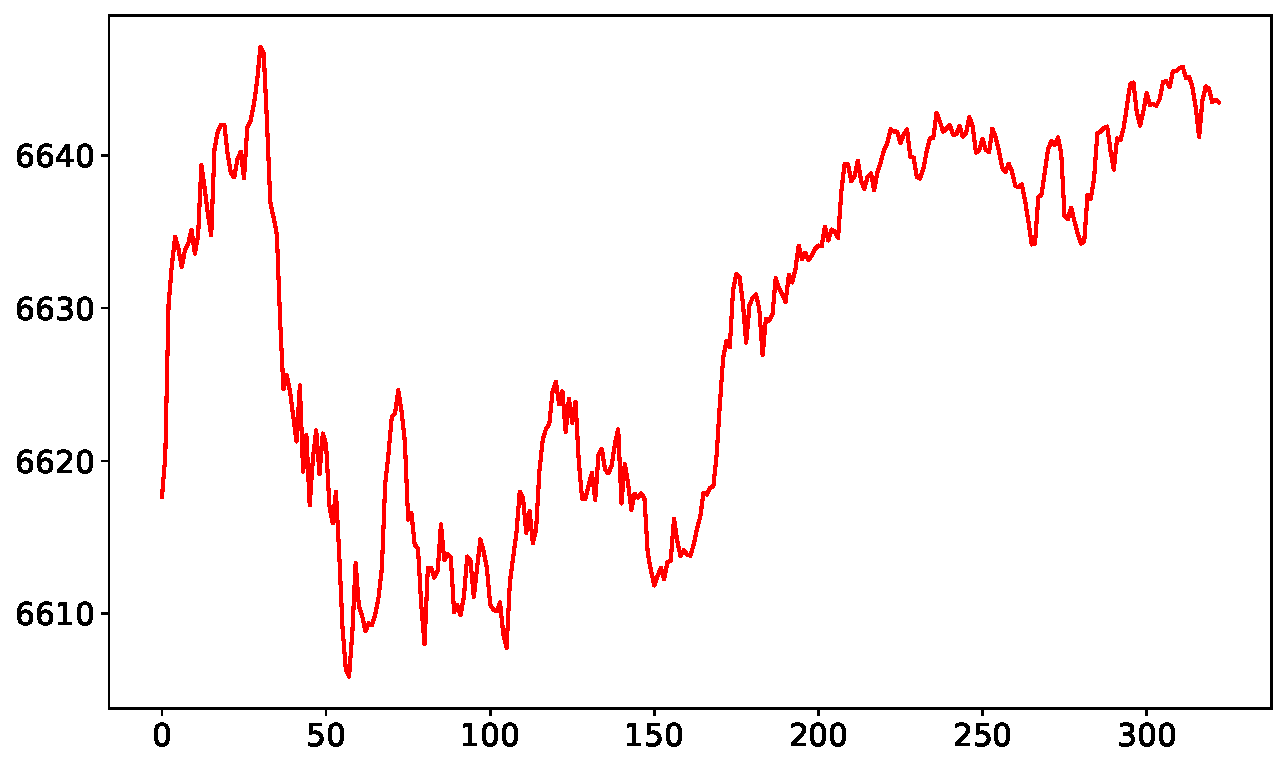
\includegraphics[width=\linewidth]{images/spot_price_sp500.pdf}
    \caption{Example spot-price time series (S\&P\,500, daily). Source: Yahoo Finance (downloaded on 26-09-2025).}
    \label{fig:spot}
\end{subfigure}
\end{figure}

This visual similarity is striking given that the two processes originate from very different mechanisms: one is a physical diffusion, the other results from the collective behaviour of many traders responding to supply and demand.

